\documentclass[a4paper,11pt]{article}
\usepackage[T2A]{fontenc}
\usepackage[warn]{mathtext}
\usepackage{mathtext}
\usepackage{amssymb}
\usepackage{amsmath}
\usepackage{listings}
\usepackage[utf8]{inputenc} 
\usepackage[russian,english]{babel}
\usepackage[pdftex,unicode,colorlinks=true,linkcolor=black]{hyperref}
\usepackage{indentfirst} 
\usepackage{tikz}
\righthyphenmin=4
\lstset{inputencoding=utf8, extendedchars=false, keepspaces = true,
   language=pascal}
\usepackage{geometry}
    \geometry{left=1.5cm}
    \geometry{right=2cm}
    \geometry{top=2cm}
    \geometry{bottom=2cm}
\begin{document}
\begin{titlepage} 

\begin{center} 
\large МИНИСТЕРСТВО ОБРАЗОВАНИЯ

РОССИЙСКОЙ ФЕДЕРАЦИИ

«МАТИ» – РОССИЙСКИЙ ГОСУДАРСТВЕННЫЙ
ТЕХНОЛОГИЧЕСКИЙ УНИВЕРСИТЕТ им. К. Э. ЦИОЛКОВСКОГО

\hline
\\[4.5cm]
\huge Отчет по курсовой работе \\[0.6cm] 
\large "ИССЛЕДОВАНИЕ АЛГОРИТМОВ СОРТИРОВКИ В СРЕДЕ OC LINUX"\\[5cm]
\begin{flushright}
\begin{tabular}{l l}
Преподаватель:&  Лидовский В.В.\\
Студент: &  Нагорный А.А.\\
Группа: & 14ИВТ-2ДБ-005\\
Вариант: & 14\\
\end{tabular}
\end{flushright}
\vfill 

{\large \today} 
{\large \LaTeX} 

\end{center} 

\thispagestyle{empty} 
\end{titlepage} 


\tableofcontents
\vfill
\begin{center}
\section{Цель исследования}
\end{center}
  Изучить различные алгоритмы сортировки, провести исследования  времени их выполнения, обозначить их как положительные, так и отрицательные стороны, 
научиться умело выбирать определенный алгоритм для конкретной задачи. Получить навык программирования на языке Pascal, 
используя среды разработки и рабочее окружение ОС Linux, набраться опыта в составлении технических отчетов с  помощью \LaTeX с использованием GNUplot для построения графиков.
\\
\\
\section{Краткая характеристика исследуемых алгоритмов сортировки}
\begin{center}
  \subsection{	Сортировка бинарным деревом}
\end{center}

  {\bfБинарным деревом} называют упорядоченную структуру данных, в которой каждому элементу поставлены в соответсвие до трех других: левый и  правый ребенок (преемник) и родитель (пред\-шественник).
Левый ребенок должен быть больше, а правый -- меньше или равен родителю. Единственный элемент, не имеющий родителя, называется корнем дерева.
 
  Если по исходной последовательности данных построить бинарное дерево, а затем вывести его элементы по правилам обхода дерева, то  полученная последовательность окажется отсортируемой.

  {\bf Правила обхода дерева}:
\begin{itemize}
    \item Обход начинается с корня, предыдущим  элементом считается верхний.
    \item Если предыдущий элемент -- верхний, то если левый преемник существует, то совершить переход к этому элементу, иначе вывод текущего элемента, и если правый преемник существует, то переход к нему, в противном случае - переход к предшественнику.
    \item Если предыдущий элемент -- левый, то вывод текущего элемента, и если правый преемник существует, то переход к правому преемнику, в противном случае - переход к предшественнику
    \item Если предыдущий элемент -- правый, то переход к предшественнику.
    \item Обход заканчивается  после вывода последнего элемента по счетчику.
\end{itemize}

В данной работе реализован рекурсивный метод обхода дерева. 

\begin{center}
  \subsection{  Метод Хоара ("Быстрая сортировка")}
\end{center}

    Суть данного метода заключается в нахождении такого элемента сортируемой последова\-тельности, который бы делил
последовательность на две части так, что слева от него находились бы элементы не меньшие его, а справа - не\ 
 большие. Поиск можно организовать разными способыми, например: 

Установим два индекса на 1-й (индекс $i$) и на последний (индекс $j$) элемент последова\-тельности. Затем,
пока элемент с индексом $i \le$ элементу с индексом $j$, будем декремен\-тировать $i$ (т.е. уменьшать на 1). 
Если же $i$-й элемент больше $j$-го, то их  меняем местами. Затем, пока $j$-й элемент $\le$ $i$-го, будем 
инкрементировать $i$ (увеличивать на 1). Если же $j$-й $\ge$ $i$-го, то менямем местами $i$ и $j$. Этот процесс
продолжаем до тех пор, пока $i \ne j$, и элемент с индексом $i = j $ - искомый. 

Далее, ищем такой же элемент для 2х полученных в результате разбиений последователь\-ностей, и продолжаем
процесс рекурсивно c вновь полученными разбиениями. Разбиения, содержащие 1 или 2 элемента, являются конечными и далее не делятся.
\\


\begin{center}
\section{Листинг исследовательской программы}
\end{center}
\scriptsize
\lstinputlisting[language=pascal]{code.pas}
\normalsize

Резульатат выполнения программы:
 \scriptsize
 \lstinputlisting{listing}
 \normalsize
 

\begin{center}
\section{Описание исследовательской программы}
\end{center}
\begin{center}
\subsection{Модули}
\end{center}

{\bf timer.o} -- объектный файл, содержащий в себе процедуры для работы с системным таймером: {\bf init\_timer()} и {\bf get\_timer()}.  
\begin{center}
\subsection{Константы}
\end{center}
{\bf maxnumber} = 70000.  Применяется в подготовке исходных данных (при заполнении массива). Обозначает максимально возможное значение элемента массива;
\linebreak 
\begin{center}
\subsection{Типы}
\end{center}

{\bf arr}. Массив целых чисел. Этим типом определяется исходный массив;

\linebreak 
{\bf menu1}. Тип, определяемый переменную перечисляемого типа (BINTREE,QSORT). Иcпользуется
при выборе алгоритма сортировки исходного массива;

\linebreak 
{\bf menu2}.  Тип, определяемый переменную перечисляемого типа (t250,t500,t1000,t4000,t8000,t16000). Иcпользуется
при выборе размера исходного массива;

\linebreak
{\bf menu3}.  Тип, определяемый переменную перечисляемого типа (SORTED,ASORTED,CHILD,RAND). Иcпользуется
при выборе типа заполнения исходного массива (упорядоченный, обратный порядок, вырожденный, случайный) ;

\linebreak 
{\bf PTreeType}.Тип, определяющий указатель на структуру {\bf rectree}. 
Применяется в алгоритме сортировки методом бинарного дерева;

\linebreak 
{\bf rectree}. Тип, определяемый как запись из: {\bf data} - числа целого типа, обозначаемого значение листа, и 3х указаителей на структуры тогоже типа : {\bf left, right, up} обозначающих узлов-соседей в алгоритме сортировки бинарным деревом.

\linebreak 
{\bf table}. Тип, определяемый как запись из: {\bf size} - числа целого типа, обозначаемого текущий  размер исходного массива , и {\bf Time} - вещественного числа, обозначающего время сортировки в миллисекундах (мс).
\\

\begin{center}
\subsection{Подпрограммы}
\end{center}
\begin{center}
\subsubsection{TestSort(a:arr)}
\end{center}

Функция проверки переданного ей массива $a$ на отсотированность: если все элементы с большими индексами больше
элементов с меньшими индексами, то $sorttest :=true$ иначе,  $sorttest :=false$ . Возвращает значения, относительно переменной $sorttest$.
\\
\begin{center}
\subsubsection{CopyArr(a,b:arr)}
\end{center}

Процедура копирования, переданного ей массива $a$ в переданный массив $b$ : в цикле каждый элемент $a$ присваивается 
элементу массива $b$ с соответствующим индексом. Затем выполняется проверка на равность элементов массивов $a$ и $b$,
со случайным индексом, максимальное значение которого не превышает размерность $a$и $b$, и, в случае ошибки, выводится 
сообщение об ошибке копирования.
\\
\begin{center}
\subsubsection{exch(var ar:arr;a,b:longint)}
\end{center}

Процедура меняет значения элементов с индексами $a$ и $b$ массива $arr$, используя временную переменную для обмена - $tmp$ 
типа longint.
\\
\begin{center}
\subsubsection{SortQuick(var ar:arr;l,u:longint)}
\end{center}

Процедура, выполняющая быструю сортировку по алгоритму Хоара. Процедура принимает следущие параметры: {\bf a} - массив, в котором проводится сортитровка,
{\bf l} - первый элемент интервала сортировки, {\bf u} - количество элементов, участвующих в сортировке. Так как алгоритм подразумевает рекурсию,
переменные $l$ и $u$ не могут быть заданы в теле процедуры явным образом. В первоначальном вызове процедуры $l=0$, a 
$u=high(ar)+1$;
\\

{\large\bfБыли добавлены рекурсивные функции для дерева. Потом добавлю}

\begin{center}
\subsubsection{SortTree(a:arr)}
\end{center}

Процедура, выполняющая сортировку методом бинарного дерева. Здесь в массиве {\bf tree} из  $high(a)+1$  элементов, каждый из которых - запись типа $rectree$, выстраивается дерево из элементов исходного массива {\bf a} по определенному правилу: левый преемник должен быть больше, а правый -- меньше или равен предшественнику. Расположение каждого элемента определяет 
переменная {\bf dir} типа $dirs$. Затем, совершается обход дерева и заполнение массива $a$ уже отсортированными данными.
\\
\begin{center}
\subsubsection{print(a:TableType;b:TableType)}
\end{center}

Процедура, выполняющая печать заранее приготовленных таблиц с результатами: $a$ содержит результаты сортировки бинарным деревом, а $b$ результаты быстрой сортировки Хоара.
\\
\begin{center}
\subsection{Блок-схема программы}
\end{center}

\begin{flushright}
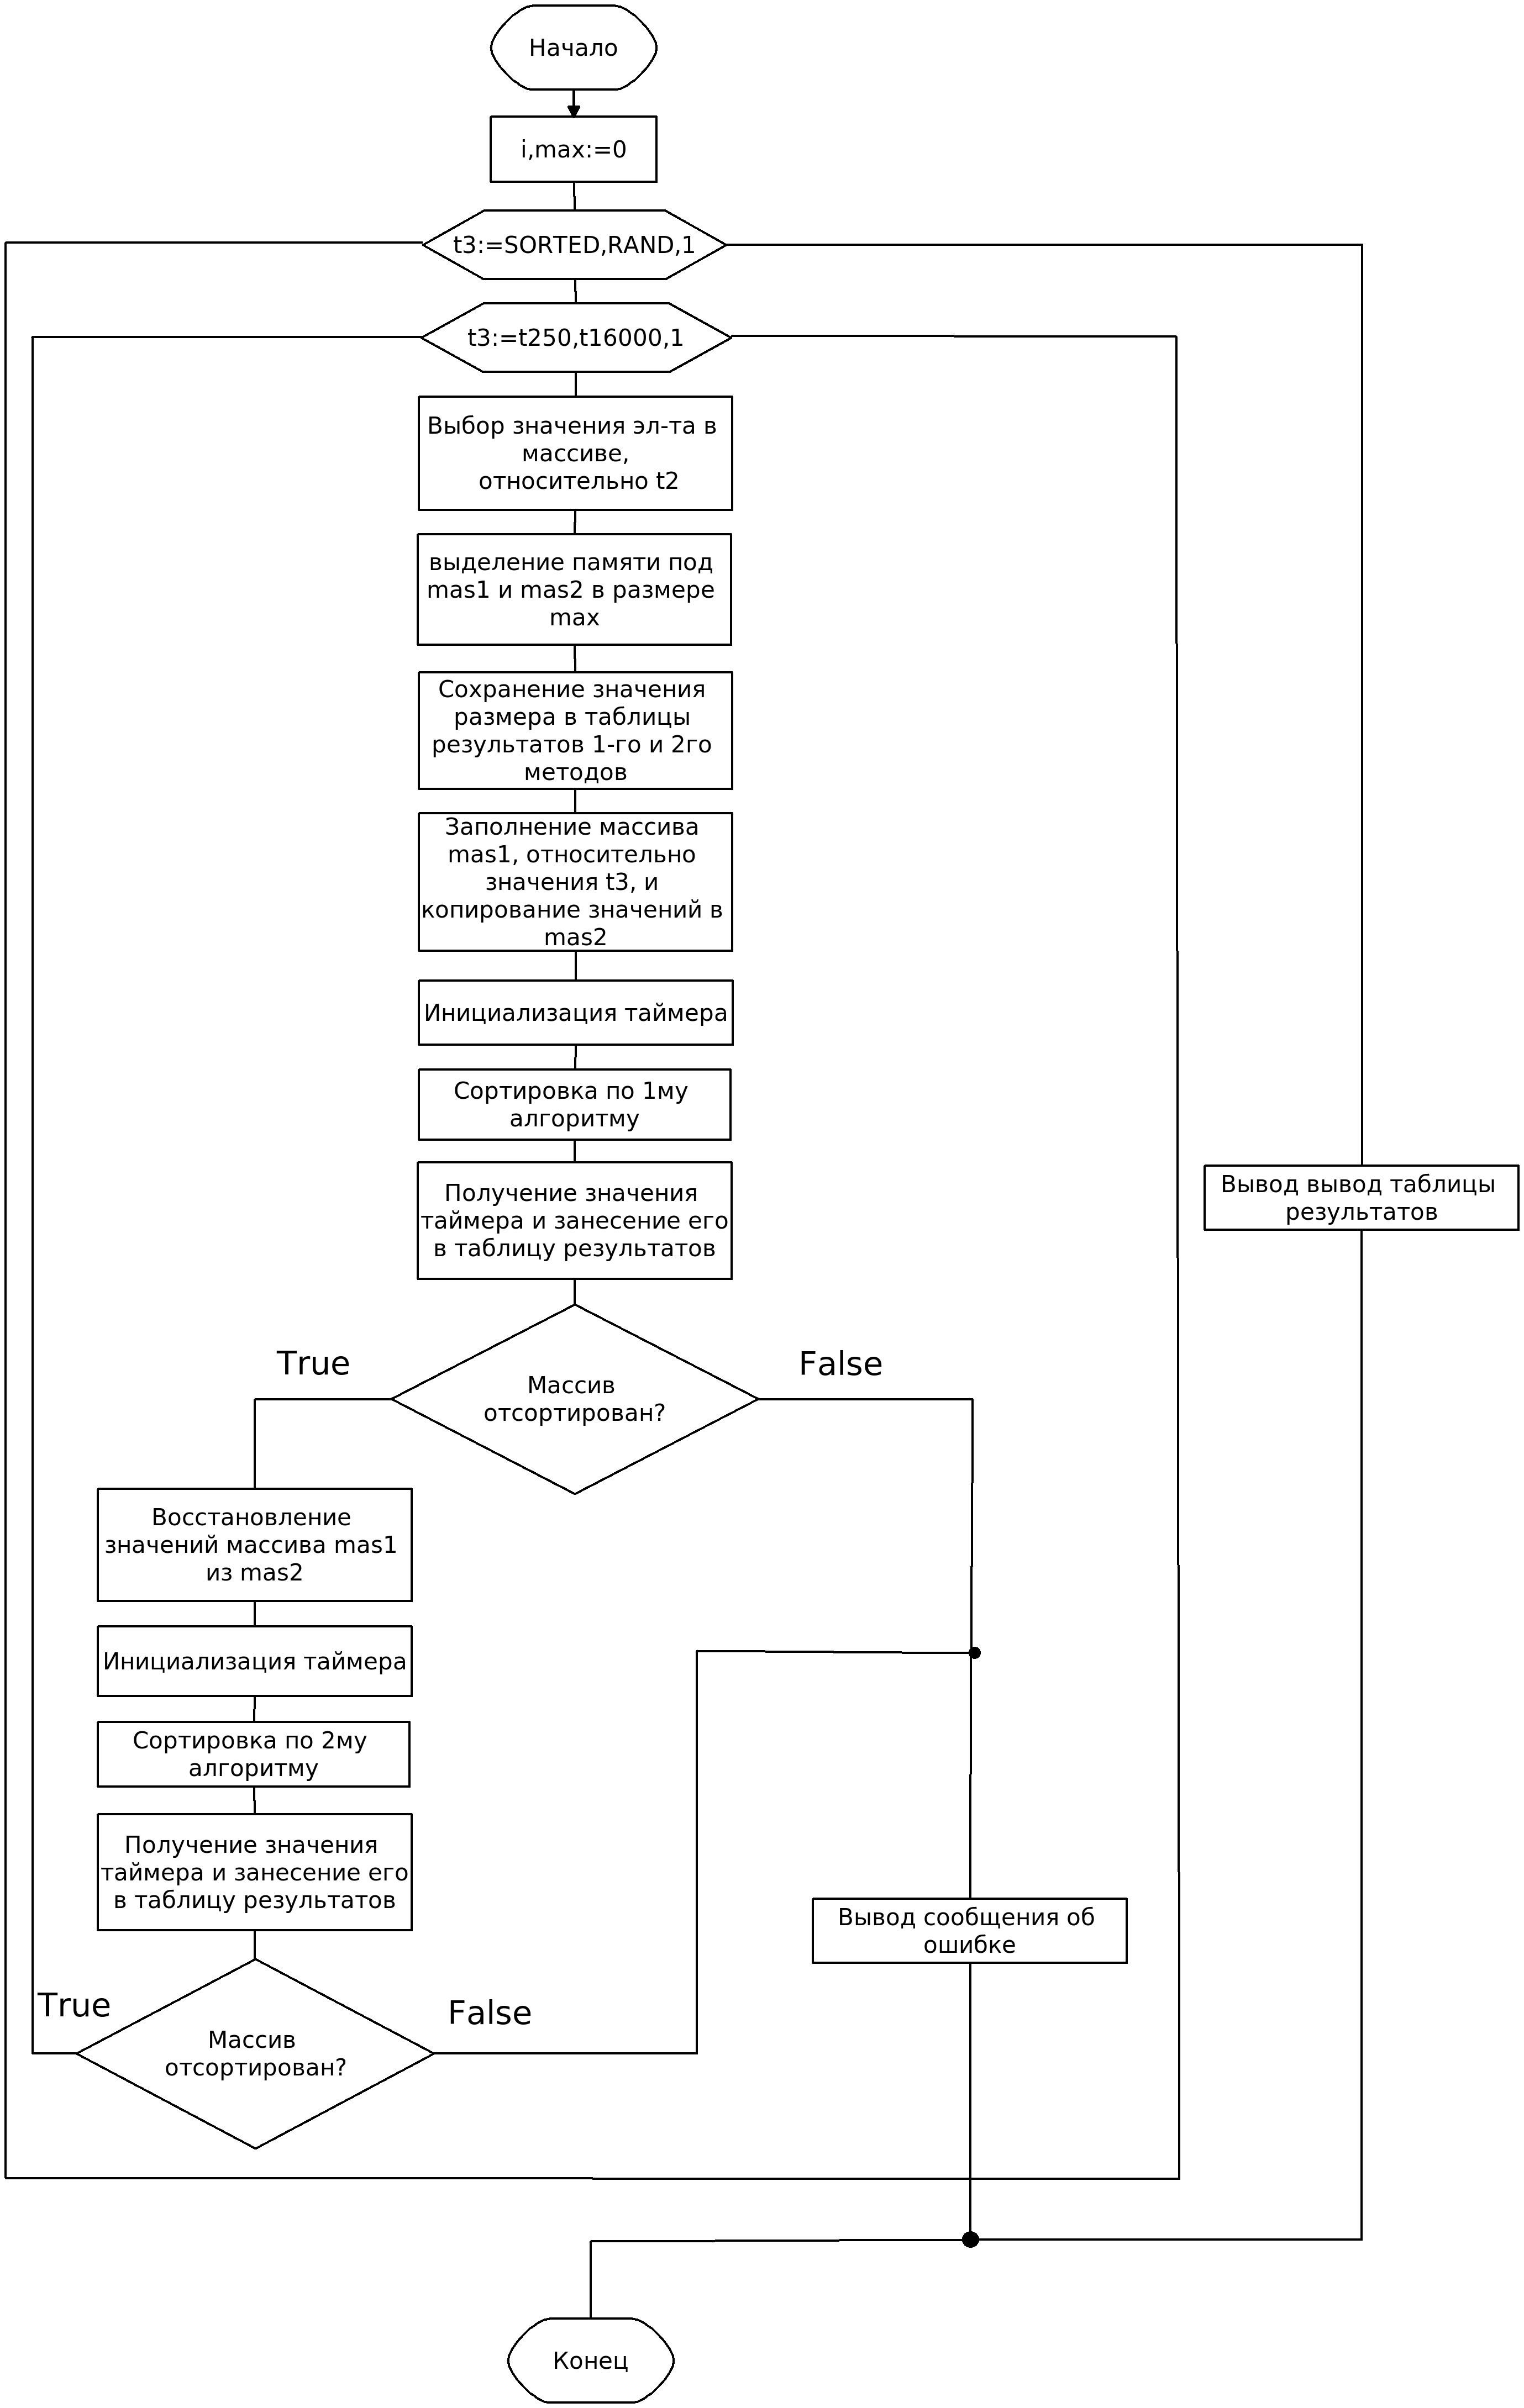
\includegraphics[height=22cm]{./scheme.png}
\end{flushright}}\\
 


\begin{center}
\section{Таблица и график результатов исследования}
\end{center}

\begin{flushright}
\begin{tabular}{|c|c|c|c|c|}
\hline
\multicolumn{5}{|c|}{Сортировка бинарным деревом / Быстрая сортировка (мс)}\\
\hline
   Размер&Упорядоченные&Обратный порядок&Вырожденные&Случайные\\
\hline
    250&0.3510 / 0.1830&0.2670 / 0.1250&0.0440 / 0.0240&0.0380 / 0.0270\\  
\hline
    500&1.3500 / 0.7170&1.0500 / 0.4880&0.1410 / 0.0740&0.0820 / 0.0600\\  
\hline
   1000&4.9090 / 1.9660&4.0690 / 1.9160&0.4530 / 0.2090&0.1870 / 0.1290\\   
\hline
   2000&16.2800 / 7.4920&15.8900 / 7.3480&1.6460 / 0.6820&0.4210 / 0.2910\\
\hline
   4000&63.6210 / 29.8030&60.6020 / 27.9920&5.9130 / 2.4730&0.8990 / 0.6400\\  
\hline
   8000&247.5150 / 119.1000&197.1270 / 96.9020&25.2400 / 9.6470&1.9190 / 1.3750\\    
\hline
  16000&987.0480 / 481.5840&409.8360 / 211.9910&108.1150 / 36.6040&4.6170 / 3.0400\\    
\hline
  $N$& $\thicksim$ $N^2$ / $N \ln^2 N$ & ~ $N \ln^2N$ / $N \ln^2N$ & ~ $N \ln(N)$ / $N$ & ~ $N$/ $N$\\ 
\hline
\end{tabular}
\end{flushright}

\begin{center}
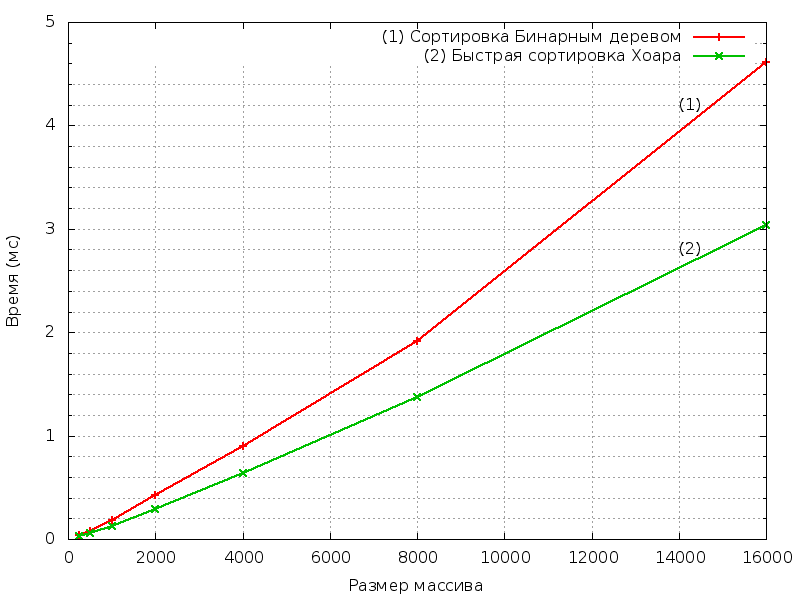
\includegraphics[height=12cm]{./graphic.png}
\end{center}\\


\begin{center}
\section{Анализ результатов эксперимента}
\end{center}

Анализируя приведенные выше результаты, можно прийти к выводу, что  {\bf сортировка бинарным деревом} и {\bf быстрая сортировка} выполняются практически за равное время для последовательнос\-тей случайных чисел одной длины. Тем не менее, уже при количестве 16000 элементов быстрая сортировка выполняется на 1.6 мсек. (0,0016 сек) быстрее, что уже является поводом для ее выбора. Кроме того, она проще, чем сортировка деревом, как с точки зрения понимания, так и реализации. Так же она не использует много памяти, не храня структуру размером $N$. Однако, рекурсивный подход может стать причиной ошибок во время реализации.
\\

\begin{center}
\section{Вывод}
\end{center}

При таком, сравнительно небольшом, значении $N$ оба метода показали себя как быстрые алгоритмы сортировки. Эти методы довольно схожи, но обладают разной сложностью реализации.

Быстрая сортировка показалась мне более удобным и оптимальным алгоритмом для сортировки числовых последовательностей. Скорость сортировки и простота реализации предоставляют возможность использовать данный алгоритм даже в крупных проектах.  Помимо этого, результат выполнения можно улучшить добавив в алгоритм рандомизированный выбор опорного элемента, что сократит время выполнения алгоритма даже для больших последовательностей.
\vfill

\begin{center}
Тестовый документ, подготовленный в \LaTeX
\end{center}
  \end{document}


